% A LaTeX (non-official) template for ISAE projects reports
% Copyright (C) 2014 Damien Roque
% Version: 0.2
% Author: Damien Roque <damien.roque_AT_isae.fr>

\documentclass[a4paper,12pt, openany]{book}
\usepackage[utf8]{inputenc}
\usepackage[T1]{fontenc}
\usepackage[frenchb]{babel} % If you write in French
%\usepackage[english]{babel} % If you write in English
\usepackage{a4wide}
\usepackage{graphicx}
\graphicspath{{images/}} % emplacement des images
\usepackage{subfig}
 \usepackage{float}
\usepackage{tikz}
\usetikzlibrary{shapes,arrows}
\usepackage{pgfplots}
\pgfplotsset{compat=newest}
\pgfplotsset{plot coordinates/math parser=false}
\newlength\figureheight
\newlength\figurewidth
\pgfkeys{/pgf/number format/.cd,
set decimal separator={,\!},
1000 sep={\,},
}
\usepackage{ifthen}
\usepackage{ifpdf}
\ifpdf
\usepackage[pdftex]{hyperref}
\else
\usepackage{hyperref}
\fi
\usepackage{color}
\hypersetup{%
colorlinks=true,
linkcolor=blue,
citecolor=black,
urlcolor=black}

\usepackage{titlesec}
\titleformat{\chapter}[hang]{\bf\huge}{\thechapter}{2pc}{}

\renewcommand{\thesection}{\Roman{section}}


\renewcommand{\baselinestretch}{1.05}
\usepackage{fancyhdr}
\pagestyle{fancy}
\fancyfoot{}
\fancyhead[LE,RO]{\bfseries\thepage}
\fancyhead[RE]{\bfseries\nouppercase{\leftmark}}
\fancyhead[LO]{\bfseries\nouppercase{\rightmark}}
\setlength{\headheight}{15pt}

\let\headruleORIG\headrule
\renewcommand{\headrule}{\color{black} \headruleORIG}
\renewcommand{\headrulewidth}{1.0pt}
\usepackage{colortbl}
\arrayrulecolor{black}

\fancypagestyle{plain}{
  \fancyhead{}
  \fancyfoot[C]{\thepage}
  \renewcommand{\headrulewidth}{0pt}
}

\makeatletter
\def\@textbottom{\vskip \z@ \@plus 1pt}
\let\@texttop\relax
\makeatother

\makeatletter
\def\cleardoublepage{\clearpage\if@twoside \ifodd\c@page\else%
  \hbox{}%
  \thispagestyle{empty}%
  \newpage%
  \if@twocolumn\hbox{}\newpage\fi\fi\fi}
\makeatother

\usepackage{amsthm}
\usepackage{amssymb,amsmath,bbm}
\usepackage{array}
\usepackage{bm}
\usepackage{multirow}
\usepackage[footnote]{acronym}

\newcommand*{\SET}[1]  {\ensuremath{\mathbf{#1}}}
\newcommand*{\VEC}[1]  {\ensuremath{\boldsymbol{#1}}}
\newcommand*{\FAM}[1]  {\ensuremath{\boldsymbol{#1}}}
\newcommand*{\MAT}[1]  {\ensuremath{\boldsymbol{#1}}}
\newcommand*{\OP}[1]  {\ensuremath{\mathrm{#1}}}
\newcommand*{\NORM}[1]  {\ensuremath{\left\|#1\right\|}}
\newcommand*{\DPR}[2]  {\ensuremath{\left \langle #1,#2 \right \rangle}}
\newcommand*{\calbf}[1]  {\ensuremath{\boldsymbol{\mathcal{#1}}}}
\newcommand*{\shift}[1]  {\ensuremath{\boldsymbol{#1}}}

\newcommand{\eqdef}{\stackrel{\mathrm{def}}{=}}
\newcommand{\argmax}{\operatornamewithlimits{argmax}}
\newcommand{\argmin}{\operatornamewithlimits{argmin}}
\newcommand{\ud}{\, \mathrm{d}}
\newcommand{\vect}{\text{Vect}}
\newcommand{\sinc}{\ensuremath{\mathrm{sinc}}}
\newcommand{\esp}{\ensuremath{\mathbb{E}}}
\newcommand{\hilbert}{\ensuremath{\mathcal{H}}}
\newcommand{\fourier}{\ensuremath{\mathcal{F}}}
\newcommand{\sgn}{\text{sgn}}
\newcommand{\intTT}{\int_{-T}^{T}}
\newcommand{\intT}{\int_{-\frac{T}{2}}^{\frac{T}{2}}}
\newcommand{\intinf}{\int_{-\infty}^{+\infty}}
\newcommand{\Sh}{\ensuremath{\boldsymbol{S}}}
\newcommand{\C}{\SET{C}}
\newcommand{\R}{\SET{R}}
\newcommand{\Z}{\SET{Z}}
\newcommand{\N}{\SET{N}}
\newcommand{\K}{\SET{K}}
\newcommand{\reel}{\mathcal{R}}
\newcommand{\imag}{\mathcal{I}}
\newcommand{\cmnr}{c_{m,n}^\reel}
\newcommand{\cmni}{c_{m,n}^\imag}
\newcommand{\cnr}{c_{n}^\reel}
\newcommand{\cni}{c_{n}^\imag}
\newcommand{\tproto}{g}
\newcommand{\rproto}{\check{g}}
\newcommand{\LR}{\mathcal{L}_2(\SET{R})}
\newcommand{\LZ}{\ell_2(\SET{Z})}
\newcommand{\LZI}[1]{\ell_2(\SET{#1})}
\newcommand{\LZZ}{\ell_2(\SET{Z}^2)}
\newcommand{\diag}{\operatorname{diag}}
\newcommand{\noise}{z}
\newcommand{\Noise}{Z}
\newcommand{\filtnoise}{\zeta}
\newcommand{\tp}{g}
\newcommand{\rp}{\check{g}}
\newcommand{\TP}{G}
\newcommand{\RP}{\check{G}}
\newcommand{\dmin}{d_{\mathrm{min}}}
\newcommand{\Dmin}{D_{\mathrm{min}}}
\newcommand{\Image}{\ensuremath{\text{Im}}}
\newcommand{\Span}{\ensuremath{\text{Span}}}

\newtheoremstyle{break}
  {11pt}{11pt}%
  {\itshape}{}%
  {\bfseries}{}%
  {\newline}{}%
\theoremstyle{break}

%\theoremstyle{definition}
\newtheorem{definition}{Définition}[chapter]

%\theoremstyle{definition}
\newtheorem{theoreme}{Théorème}[chapter]

%\theoremstyle{remark}
\newtheorem{remarque}{Remarque}[section]

%\theoremstyle{plain}
\newtheorem{propriete}{Propriété}[chapter]
\newtheorem{exemple}{Exemple}[chapter]

\newtheorem{question}{Question}[chapter]

\parskip=5pt
%\sloppy

\begin{document}

%%%%%%%%%%%%%%%%%%
%%% First page %%%
%%%%%%%%%%%%%%%%%%

\begin{titlepage}
\begin{center}


\includegraphics[width=0.6\textwidth]{ensimag_logo.png}\\[1cm]

{\large Ensimag MMIS 3A}\\[0.5cm]

{\large Ondelettes et applications à l'image}\\[0.5cm]

% Title
\rule{\linewidth}{0.5mm} \\[0.4cm]
{ \huge \bfseries Compte-Rendu du lab 2\\[0.4cm] }
\rule{\linewidth}{0.5mm} \\[1.5cm]

% Author and supervisor
\noindent
\begin{minipage}{0.4\textwidth}
  \begin{flushleft} \large
    \emph{Auteurs :}\\
    % M\up{me} Prénom \textsc{Nom}\\
    M. Antonin \textsc{Klopp-Tosser} \\
    M. Yoan \textsc{Souty} \\
  \end{flushleft}
\end{minipage}%
\begin{minipage}{0.4\textwidth}
  \begin{flushright} \large
    \emph{Encadrants :} \\
    M\up{me} Valérie \textsc{Perrier} \\

    % Dr.~Prénom \textsc{Nom}
  \end{flushright}
\end{minipage}

\vfill

% Bottom of the page
{\large \today}

\end{center}
\end{titlepage}

%%%%%%%%%%%%%%%%%%%%%%%%%%%%%
%%% Non-significant pages %%%
%%%%%%%%%%%%%%%%%%%%%%%%%%%%%


%%%%%%%%%%%%%%%%%%%%%%%%%%%%%%%%%%%%%%%%%%%%
%%% Content of the report and references %%%
%%%%%%%%%%%%%%%%%%%%%%%%%%%%%%%%%%%%%%%%%%%%

\pagestyle{fancy}


\tableofcontents

\clearpage

\listoffigures

\clearpage

\section{Exercice 1}
Les figures suivantes présentent les \textit{scaling functions} et les \textit{wavelet functions} associées des familles suivantes :

\begin{itemize}
  \item base de Haar
  \item Spline Battle-Lemaire
  \item famille à support compact Daubechies
\end{itemize}

\begin{figure}[H]
  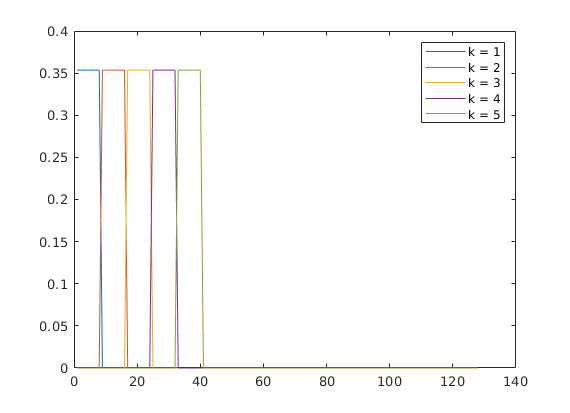
\includegraphics[width=0.5\textwidth]{HaarMultipleScaleFather}\hfill
  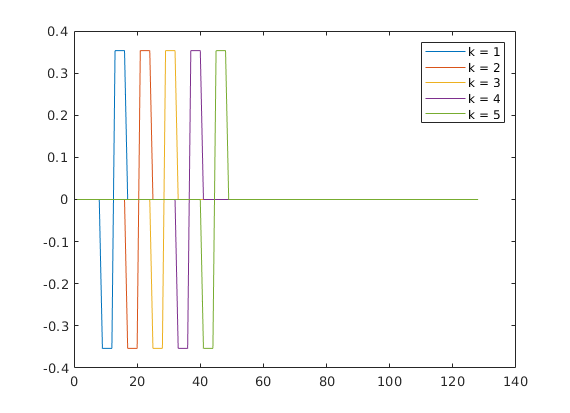
\includegraphics[width=0.5\textwidth]{HaarMultipleScaleMother}
  \subfloat[\label{fig:haar_scaling} Scaling functions.]{\hspace{.5\linewidth}}
  \subfloat[\label{fig:haar_wavelets} Wavelets.]{\hspace{.5\linewidth}}
  \caption{Résultat pour la base de Haar, $J=4$}
  \label{fig:haar_family}
\end{figure}

\begin{figure}[H]
  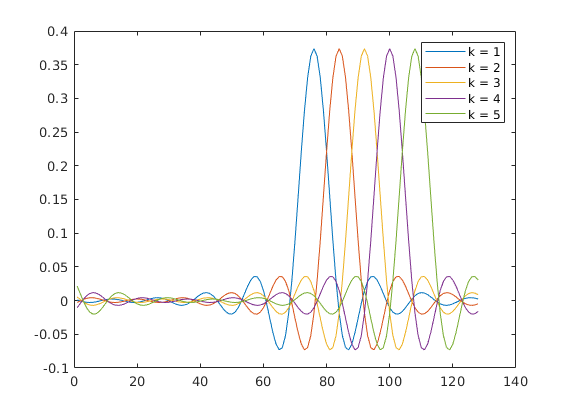
\includegraphics[width=0.5\textwidth]{BattleMultipleScaleFather}\hfill
  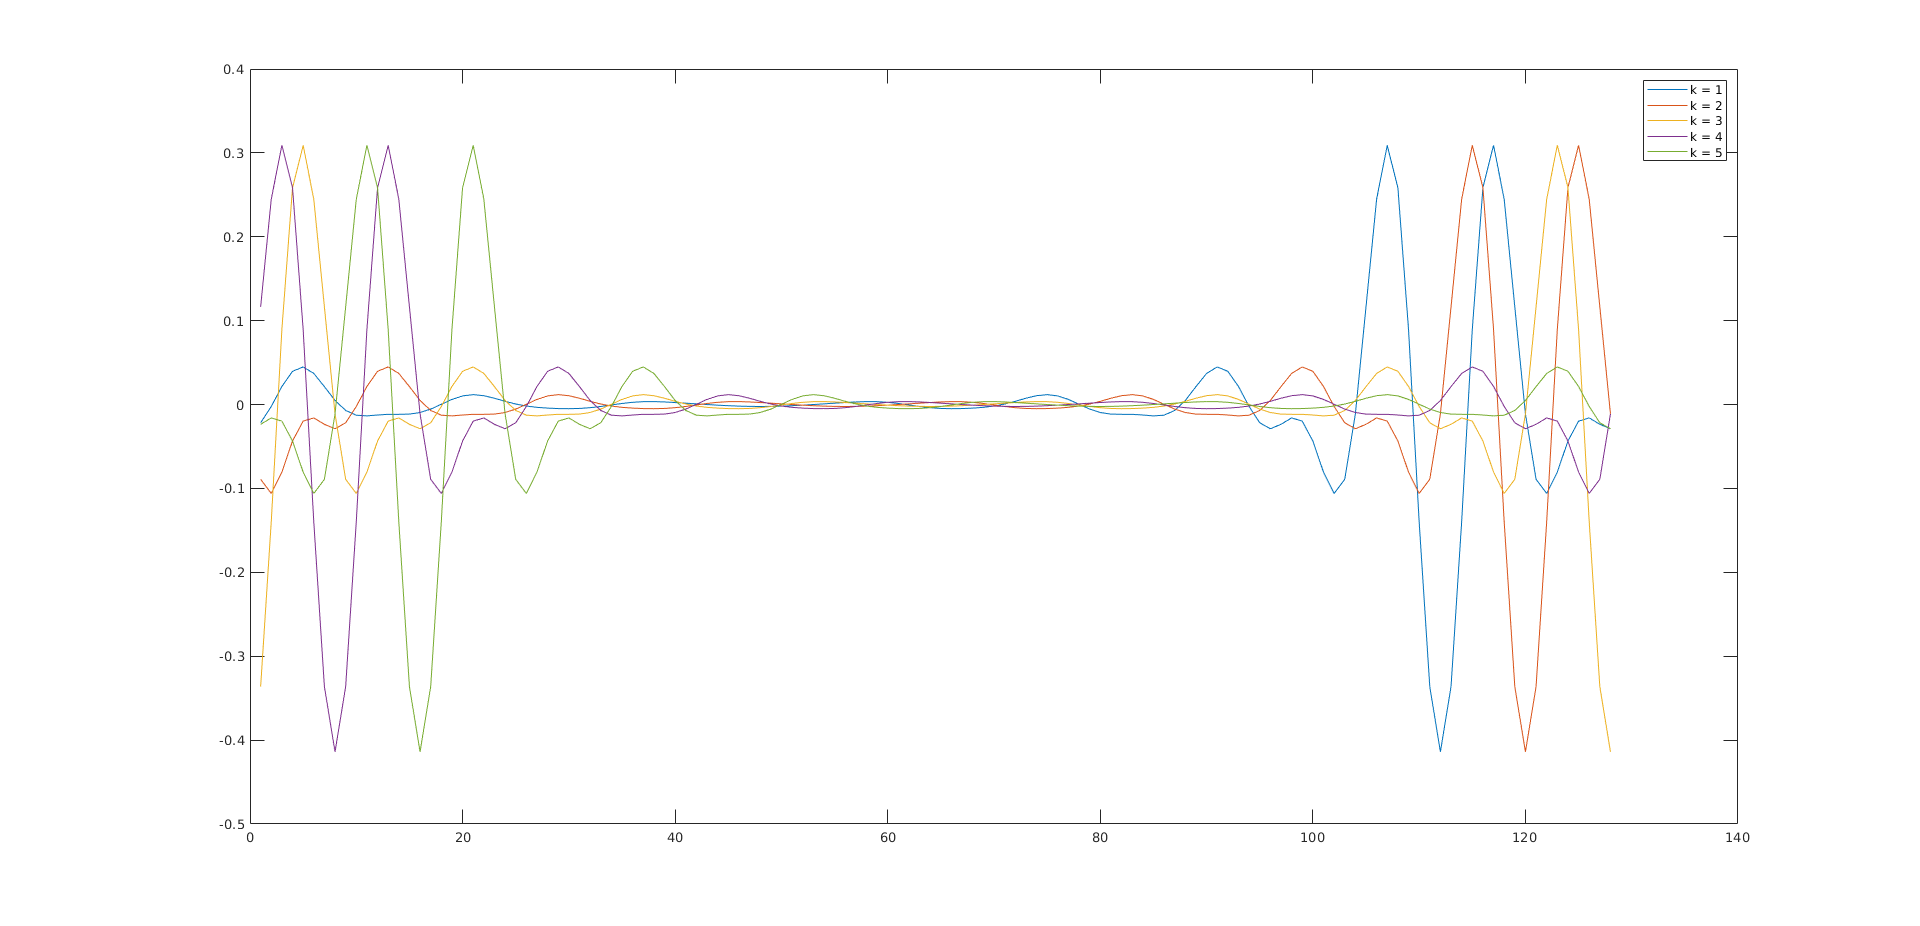
\includegraphics[width=0.5\textwidth]{BattleMultipleScale}
  \subfloat[\label{fig:spline_scaling} Scaling functions.]{\hspace{.5\linewidth}}
  \subfloat[\label{fig:spline_wavelets} Wavelets.]{\hspace{.5\linewidth}}
  \caption{Résultat pour la base spline Battle-Lemaire, $J=4$}
  \label{fig:spline_family}
\end{figure}

\begin{figure}[H]
  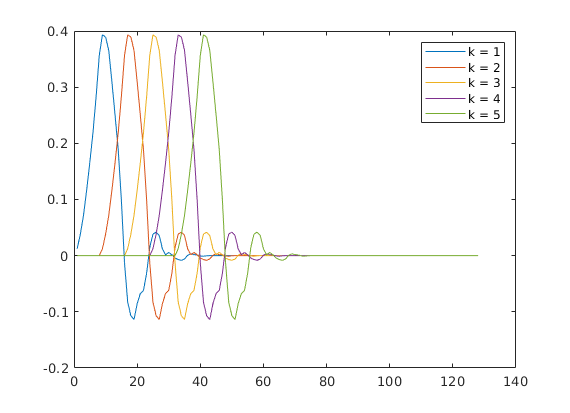
\includegraphics[width=0.5\textwidth]{DaubechiesMultipleScaleFather}\hfill
  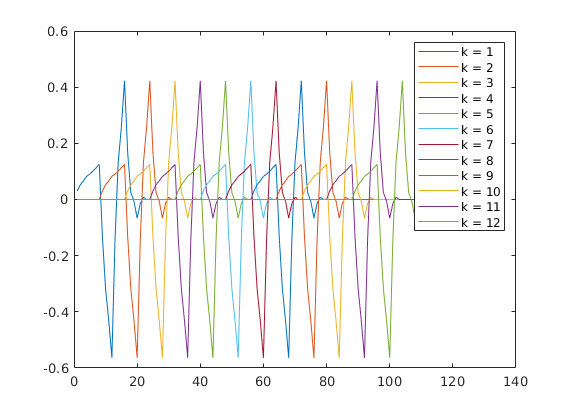
\includegraphics[width=0.5\textwidth]{DaubechiesMultipleScale}
  \subfloat[\label{fig:deb_scaling} Scaling functions.]{\hspace{.5\linewidth}}
  \subfloat[\label{fig:deb_wavelets} Wavelets.]{\hspace{.5\linewidth}}
  \caption{Résultat pour la base de Daubechies, $J=4$}
  \label{fig:deb_family}
\end{figure}

La base de Haar a l'avantage de proposer un algorithme de décomposition (et de reconstruction) en complexité linéaire ($O(N)$).

Les autres familles permettent d'avoir une meilleure compression en gardant le même nombre de coefficients.


\section{Exercice 2 : compression de signaux 1D}
\subsection{Compression de signaux}

Pour reconstruire un signal de taille $n$ à partir des coefficients en ondelettes, on prend en paramètre un taux de compression $\tau \in [0,1]$ , et l'on ne garde que $(1-tau)$\% des plus grands coefficients.

Voici les résultats de compression pour les fonctions $f: x \mapsto \sqrt{| \cos{2\pi  x}|}$, et pour deux familles de signaux 1D disponibles avec la commande \texttt{MakeSignal} : \textit{Sing, Riemann, Doppler}. Pour chaque signal, on affiche de haut en bas, la fonction d'origine, les coefficients des ondelettes et la fonction reconstruite.

Pour la base de Haar, on utilise un nombre d'échelles à 8, un moment dissipant de 4 = $\frac{8}{2}$, et un moment dissipant de 5 pour la famille Battle.

\begin{figure}[H]
  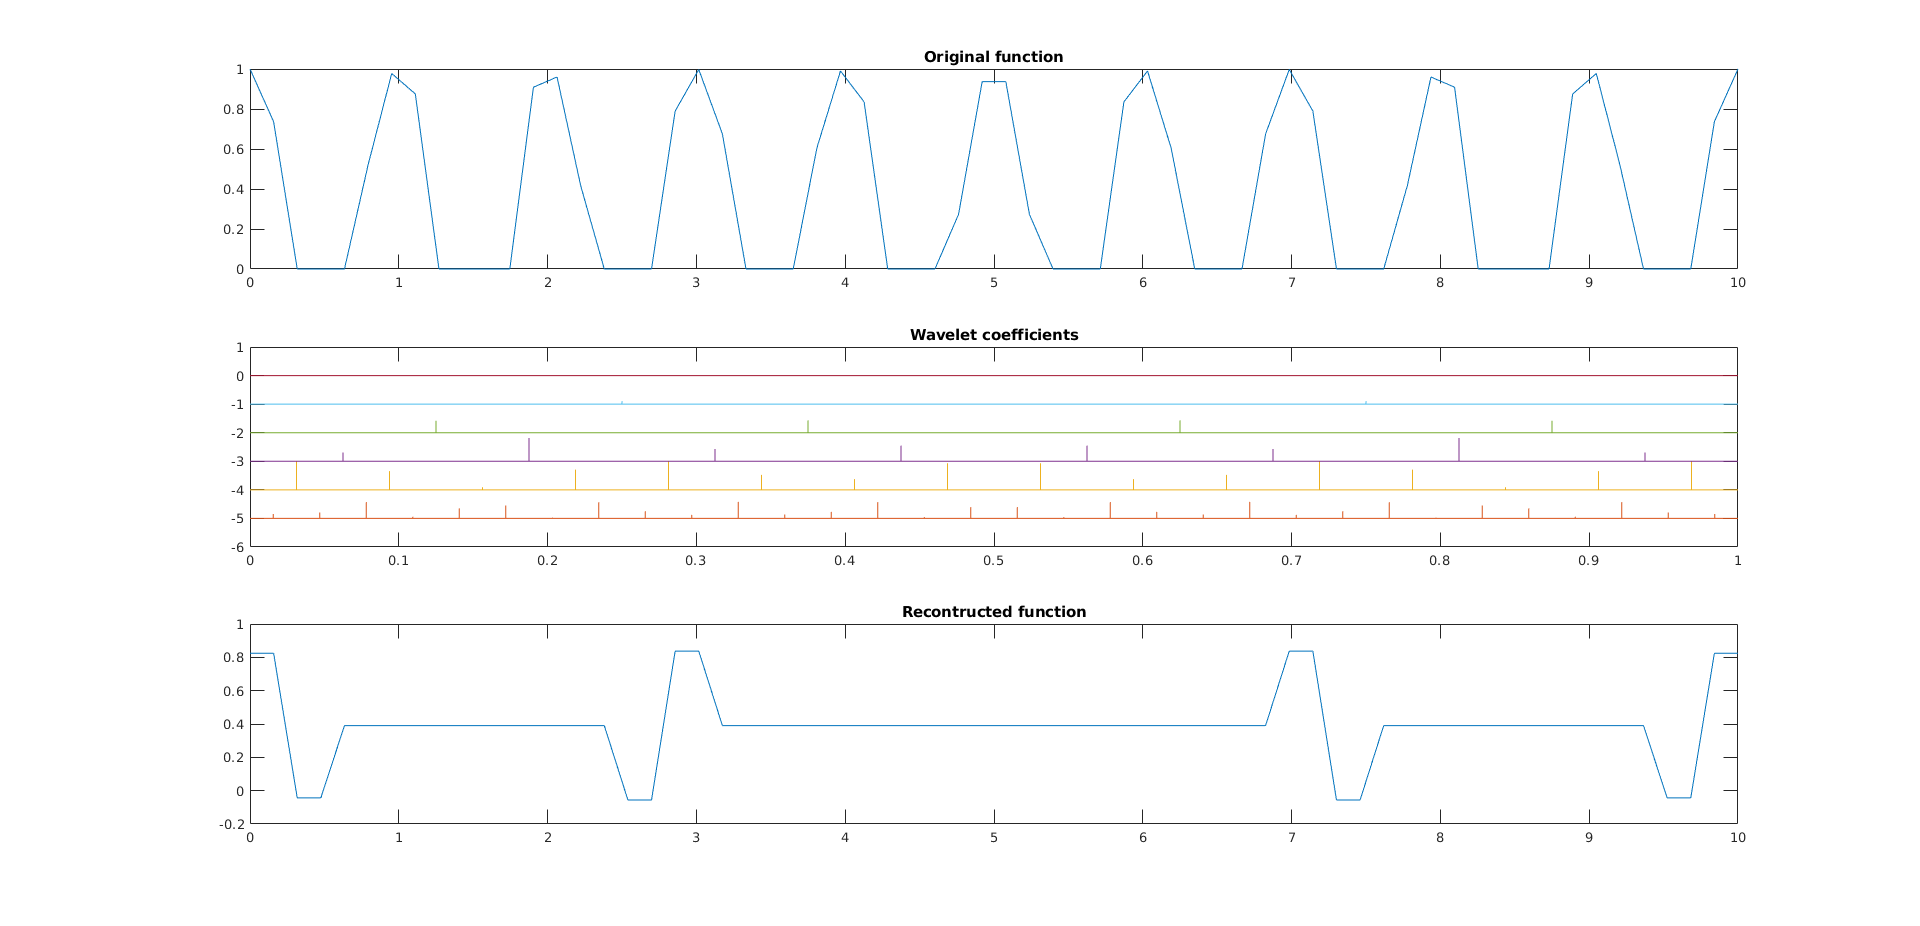
\includegraphics[width=\textwidth]{compressHaar64points_taux_0_92}
  \caption{Fonction $f$ compressée avec la base de Haar, $\tau=0.92, n=64$}
\end{figure}

\begin{figure}[H]
  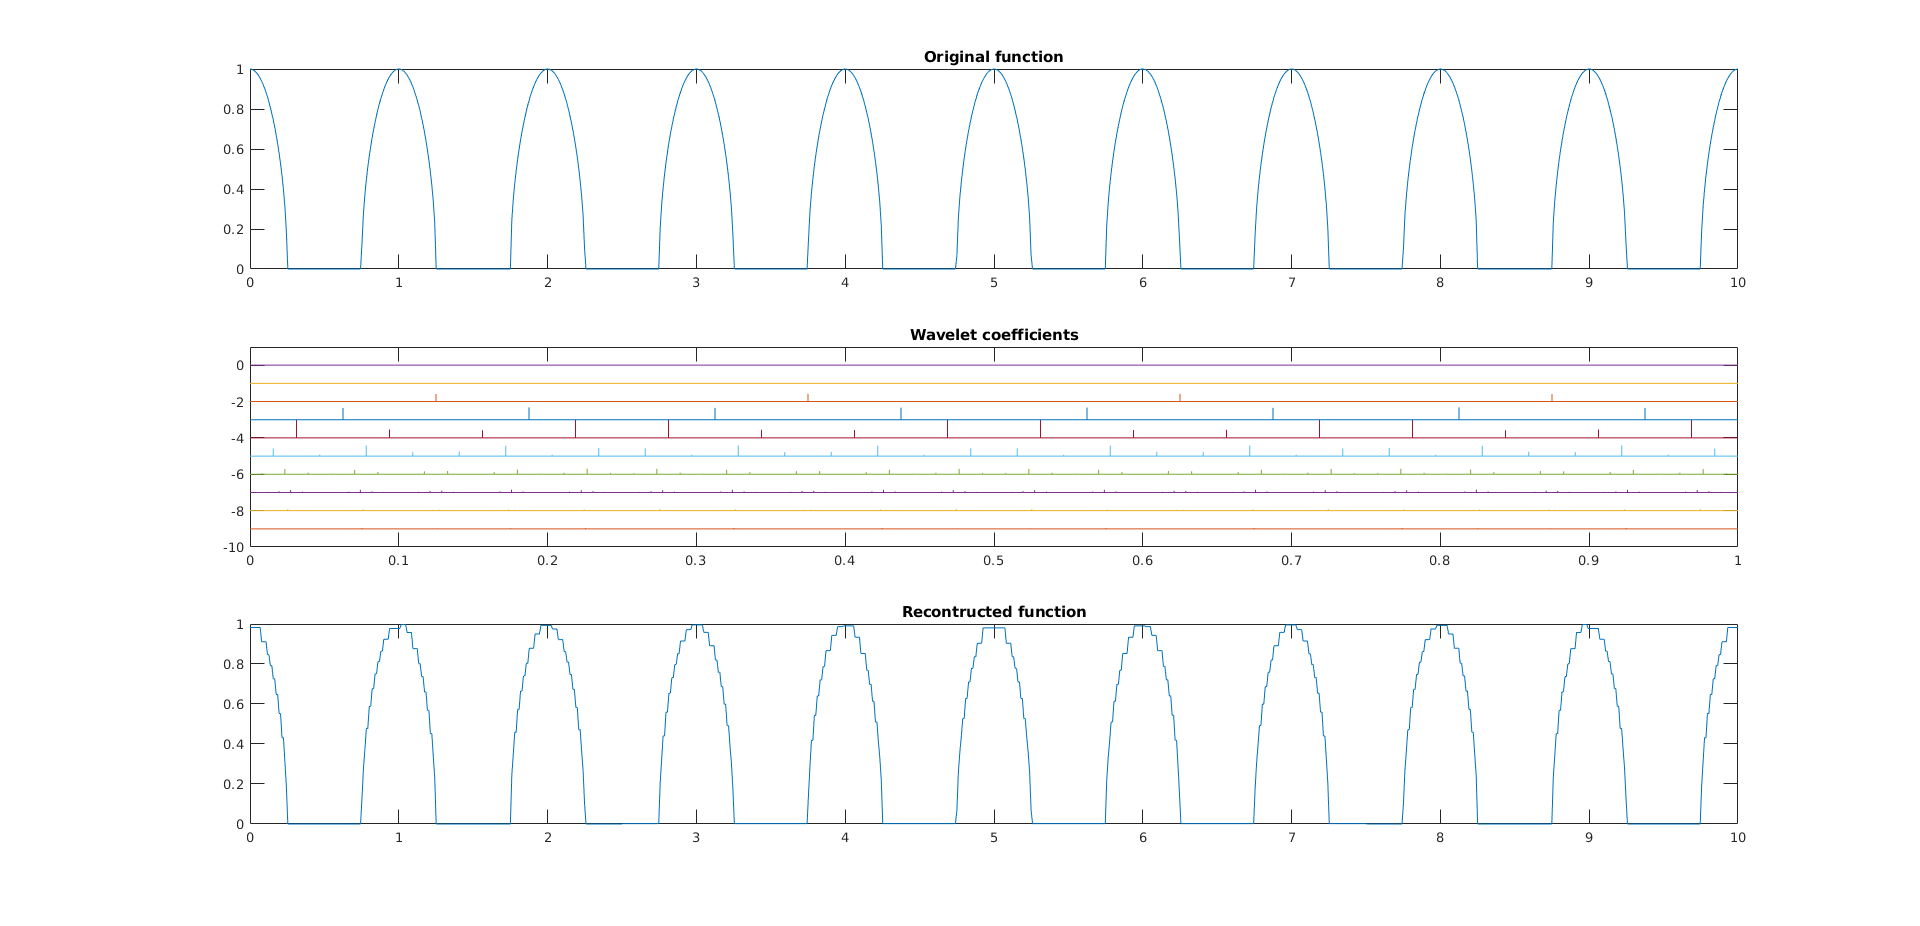
\includegraphics[width=\textwidth]{compressHaar1024points_taux0_6}
  \caption{Fonction $f$ compressée avec la base de Haar, $\tau=0.6, n=1024$}
\end{figure}

\begin{figure}[H]
  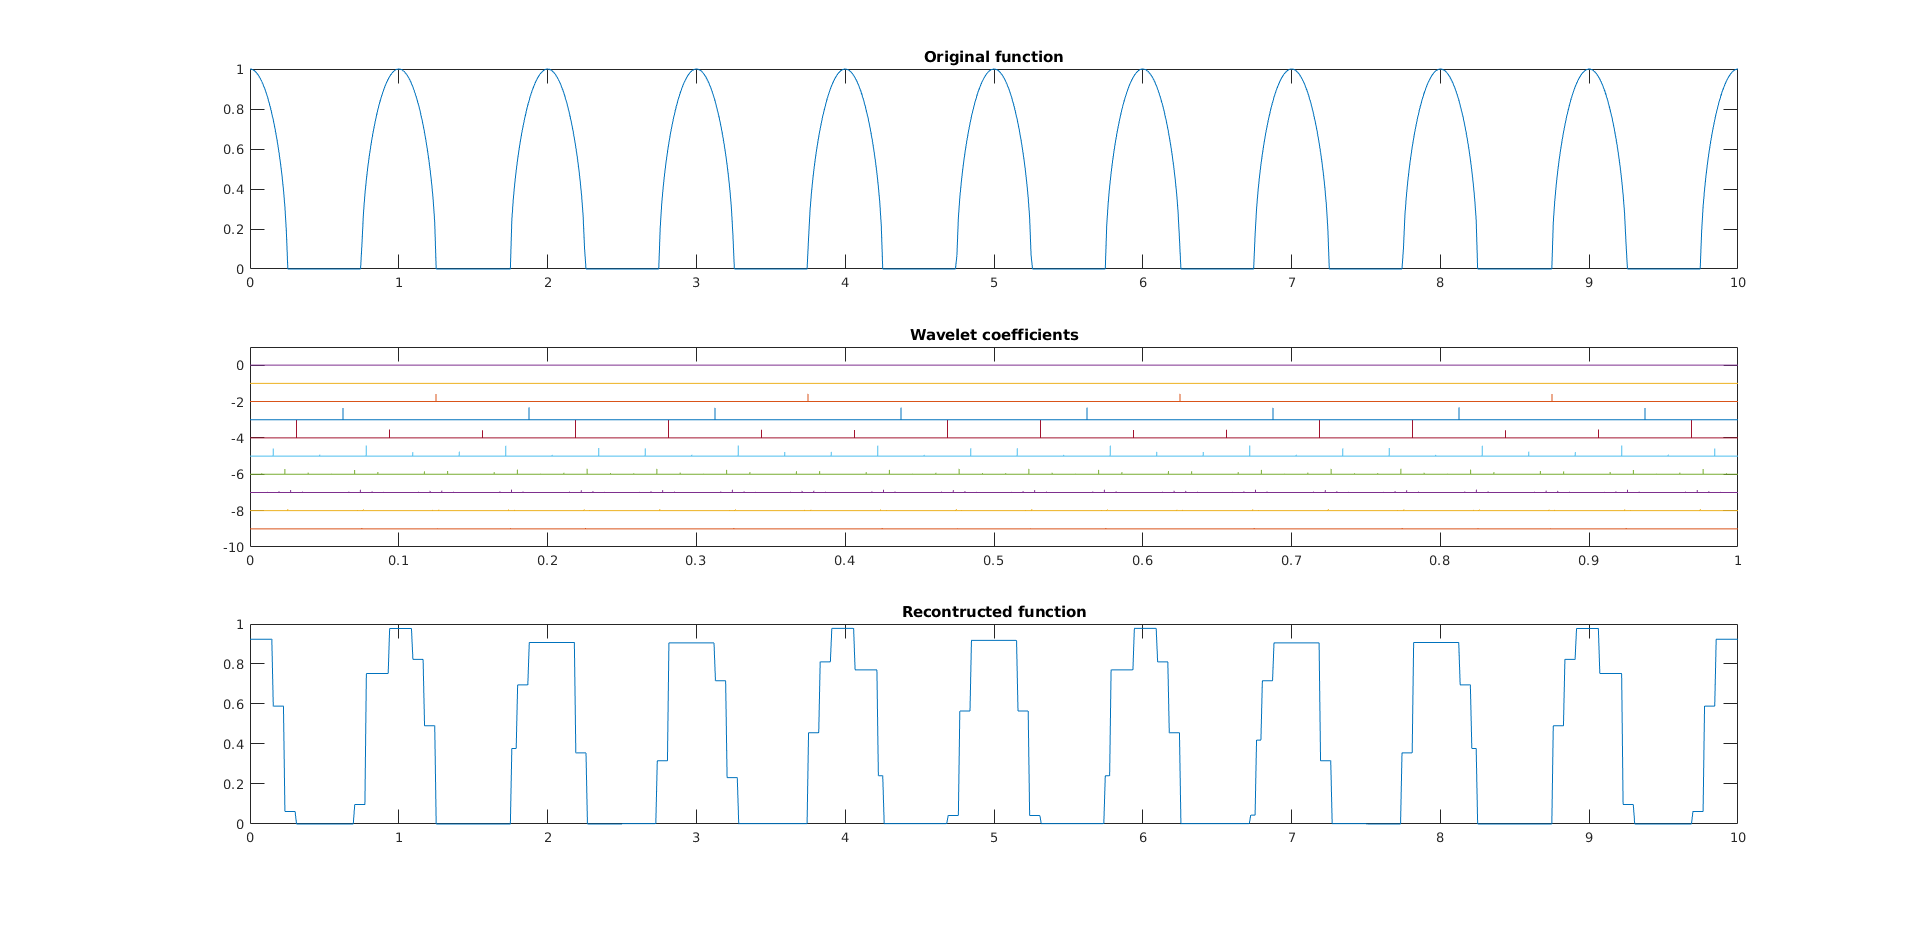
\includegraphics[width=\textwidth]{compressHaar1024points_taux0_92}
  \caption{Fonction $f$ compressée avec la base de Haar, $\tau=0.92, n=1024$}
\end{figure}

\begin{figure}[H]
  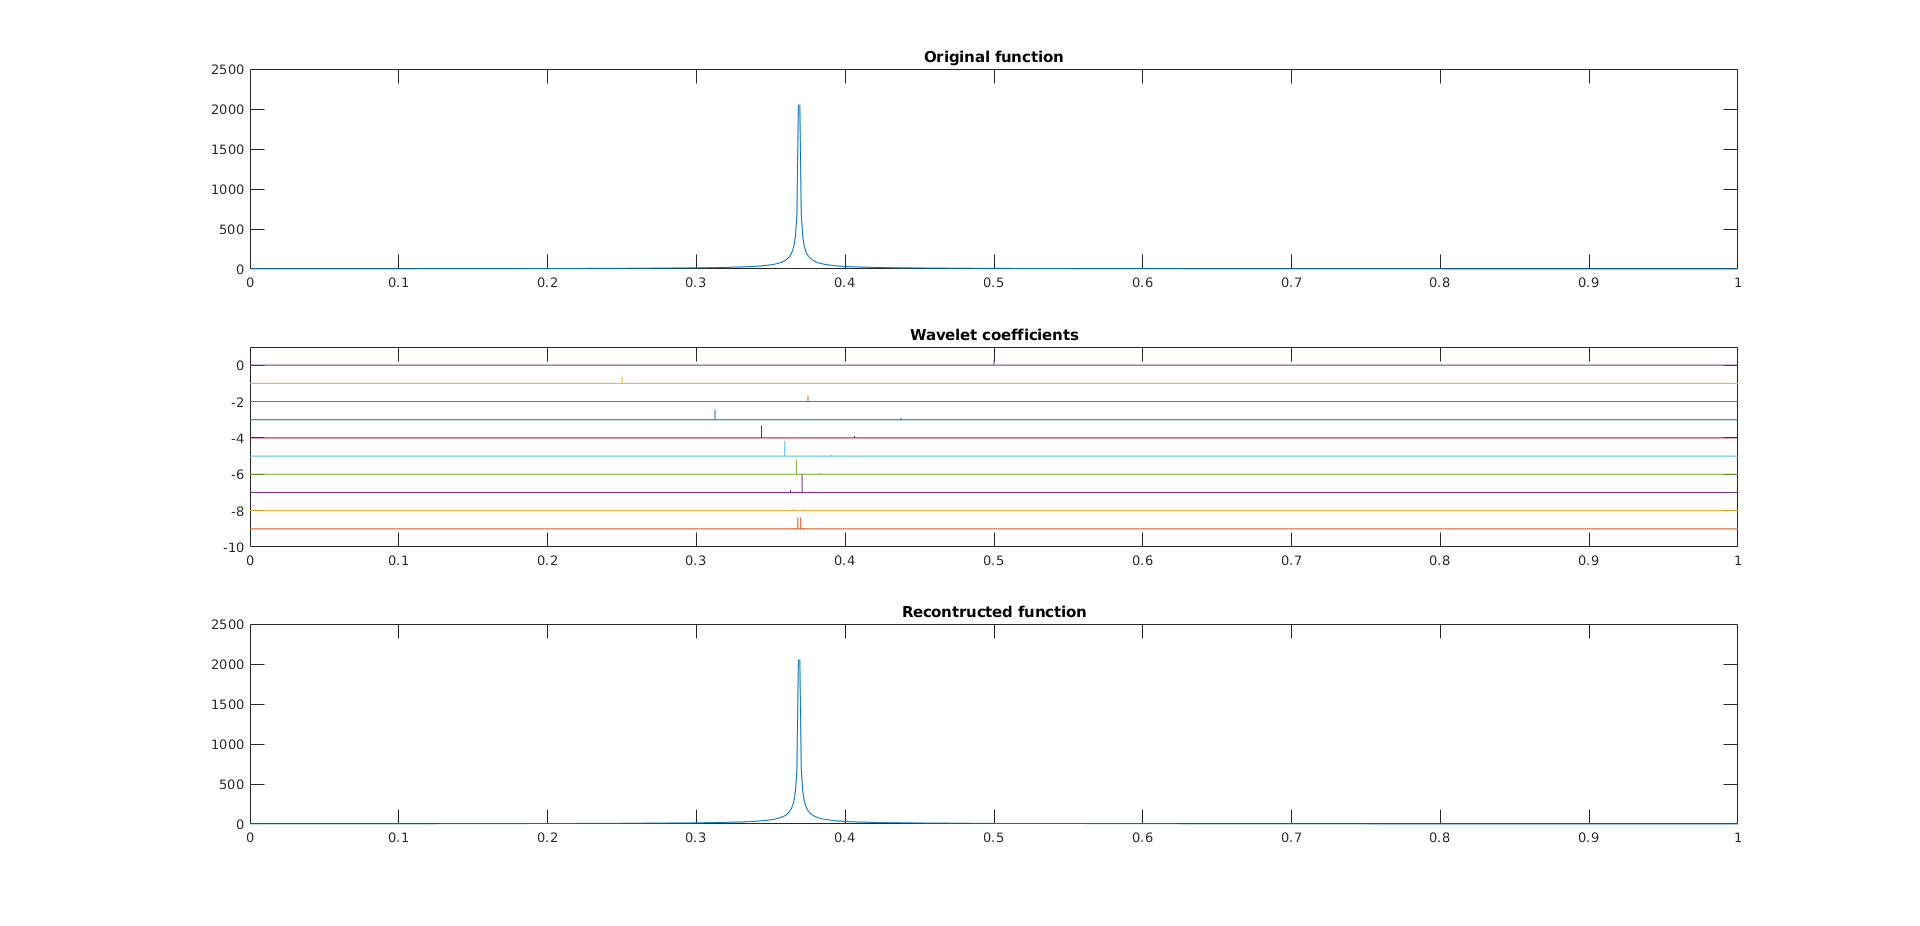
\includegraphics[width=\textwidth]{Sing_compression0_92Haar}
  \caption{Signal \textit{Sing} compressé avec la base de Haar, $\tau=0.92, n=1024$}
\end{figure}

\begin{figure}[H]
  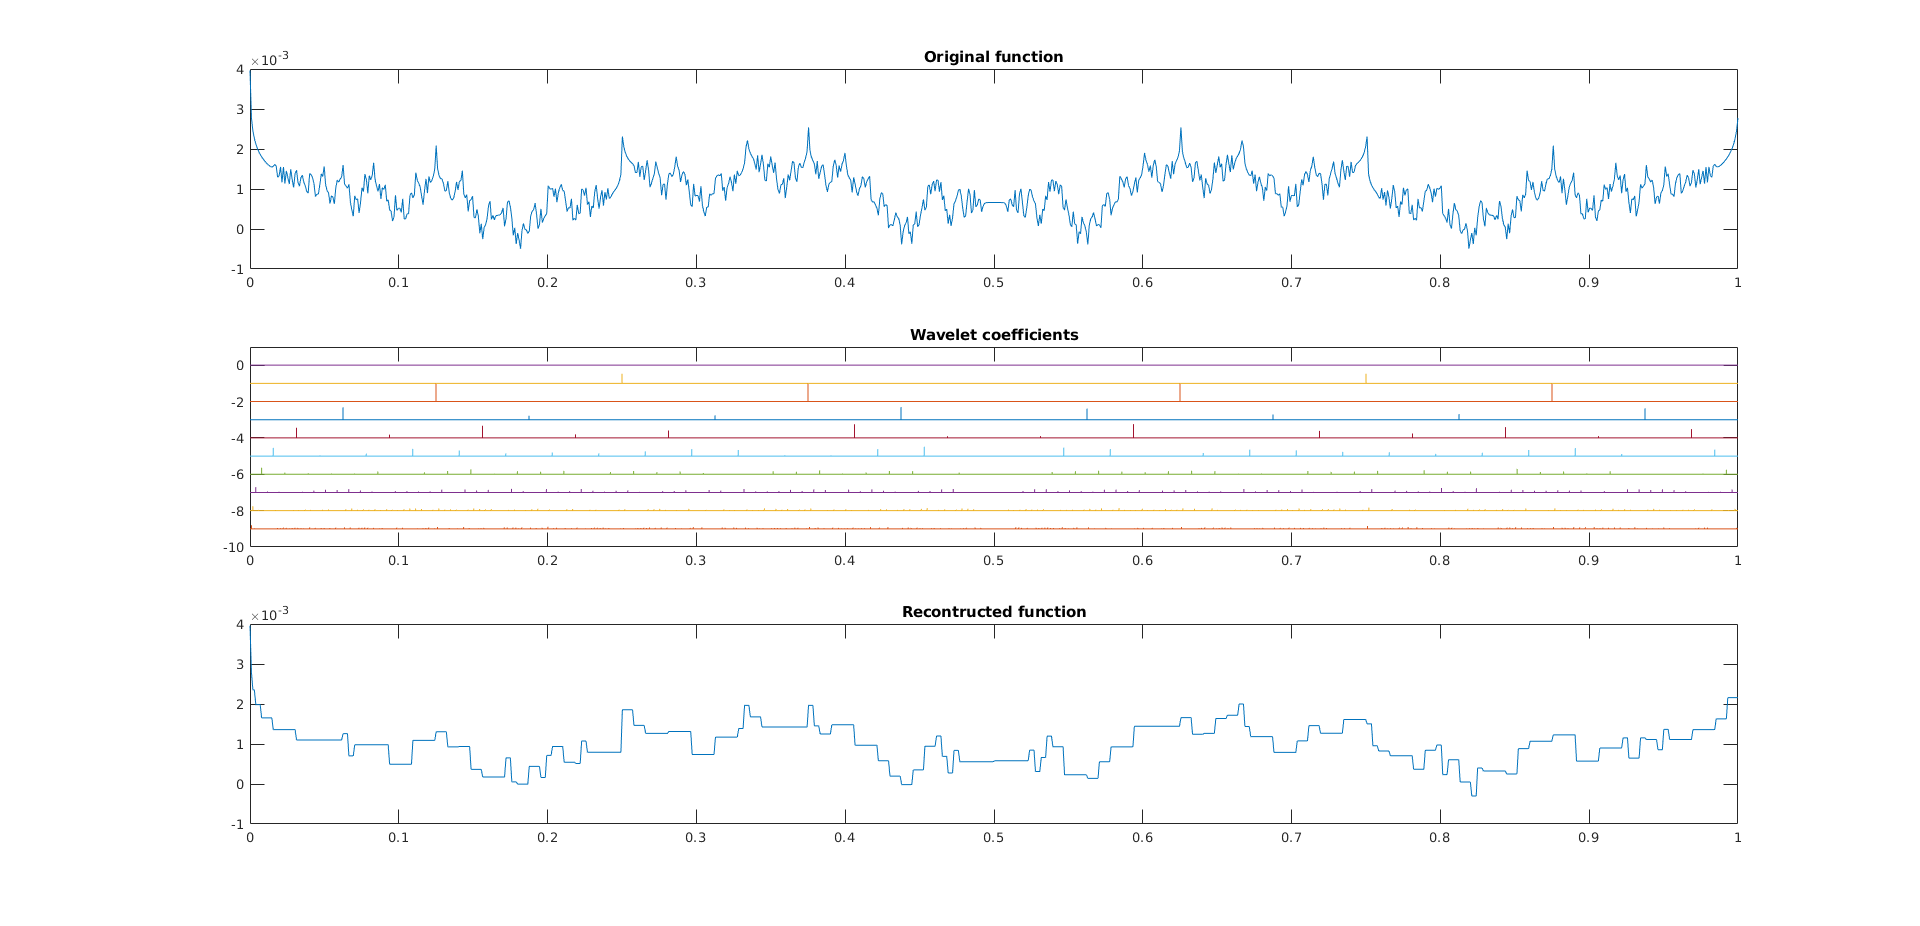
\includegraphics[width=\textwidth]{Riemann_compression_0_92Haar}
  \caption{Signal \textit{Riemann} compressé avec la base de Haar, $\tau=0.92, n=1024$}
\end{figure}

Pour le signel Doppler, nous avons affiché les compressions avec les trois familles d'ondelettes orthogonales précédemment citées.
\begin{figure}[H]
  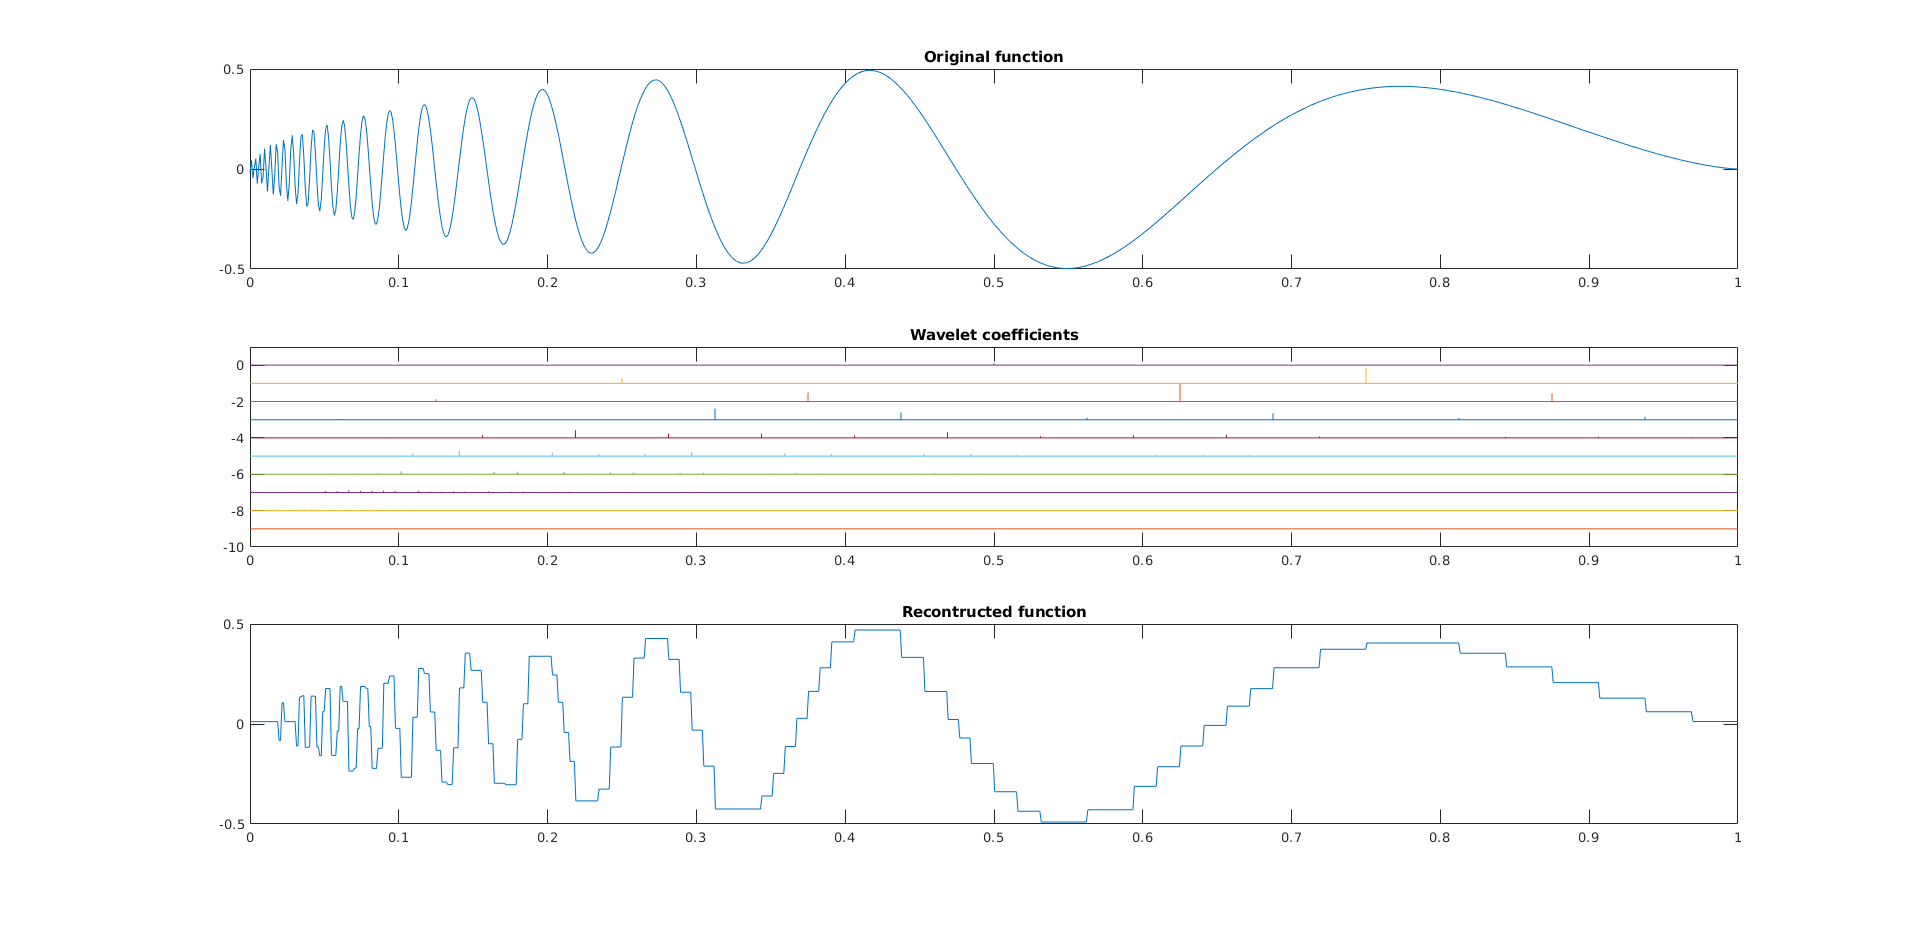
\includegraphics[width=\textwidth]{Doppler_compression_0_92Haar}
  \caption{Signal \textit{Doppler} compressé avec la base de Haar, $\tau=0.92, n=1024$}
\end{figure}

\begin{figure}[H]
  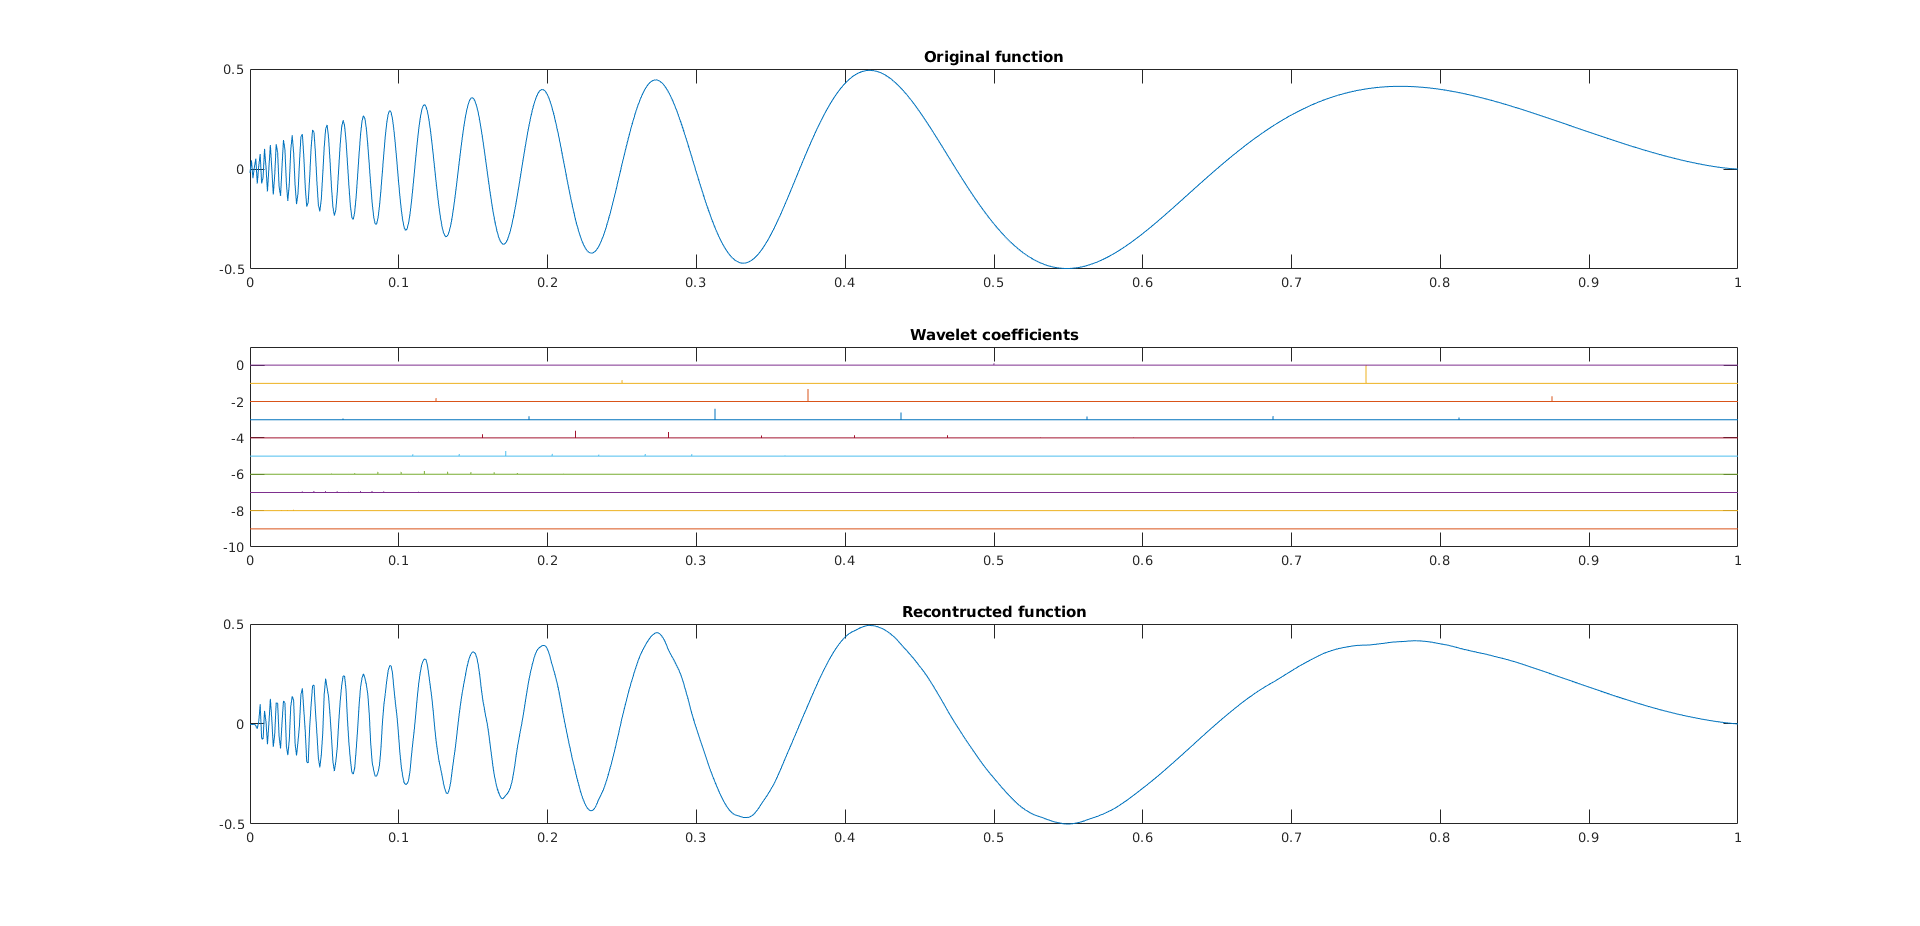
\includegraphics[width=\textwidth]{Doppler_compression_0_92Daubechies}
  \caption{Signal \textit{Doppler} compressé avec la base de Daubechies, $\tau=0.92, n=1024$}
\end{figure}

\begin{figure}[H]
  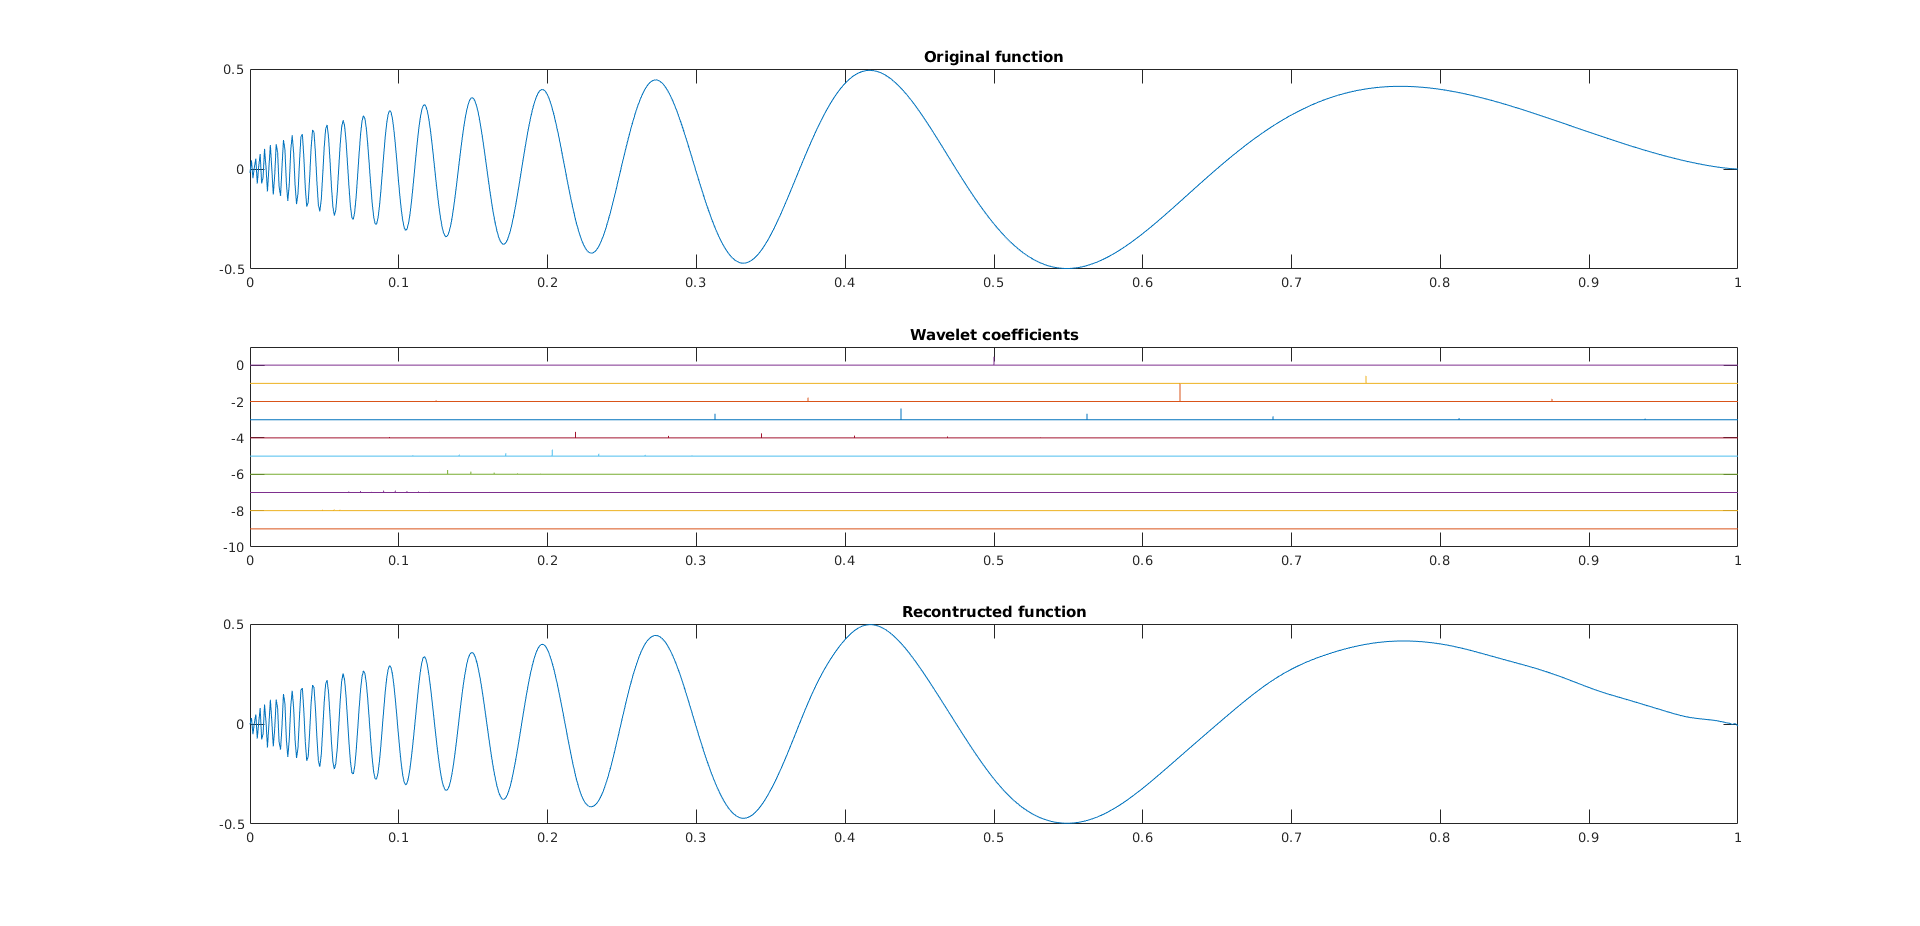
\includegraphics[width=\textwidth]{Doppler_compression_0_92Battle}
  \caption{Signal \textit{Doppler} compressé avec la base de Battle, $\tau=0.92, n=1024$}
\end{figure}

On constate qu'appliquer un taux de compression important sur un signal avec la base de Haar supprime un nombre important d'informations, alors qu'utiliser la base de Daubechies ou Battle permet \textit{a priori} de conserver plus d'informations.

\subsection{Analyse de l'erreur}
Nous avons tracé la courbe Log-Log de l'erreur $l_2$ en fonction du taux de compression $\tau$.

\begin{figure}[H]
  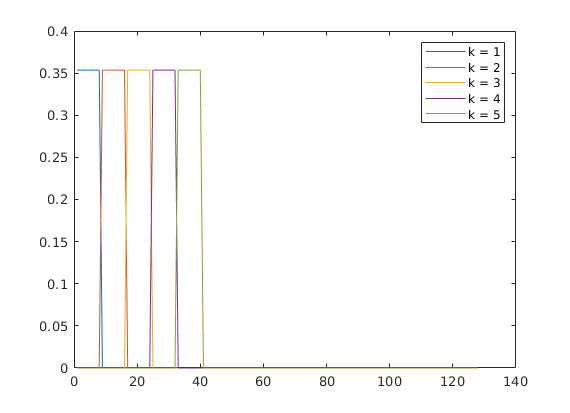
\includegraphics[width=0.4\textwidth]{HaarMultipleScaleFather}\hfill
  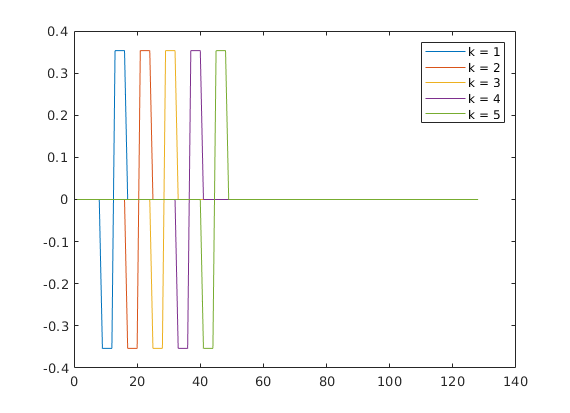
\includegraphics[width=0.4\textwidth]{HaarMultipleScaleMother}\hfill
  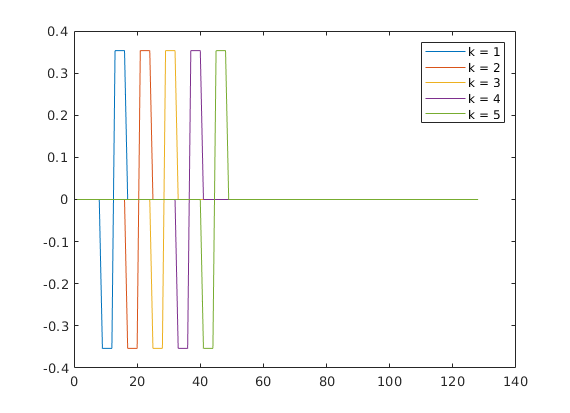
\includegraphics[width=0.4\textwidth]{HaarMultipleScaleMother}\hfill
  \subfloat[\label{fig:haar_scaling} Scaling functions.]{\hspace{.5\linewidth}}
  \subfloat[\label{fig:haar_wavelets} Wavelets.]{\hspace{.5\linewidth}}
  \caption{Signal \textit{Doppler} compressé avec la base de Haar, $\tau=0.92, n=1024$}
\end{figure}

%
% \appendix
%
% \bibliographystyle{authoryear-fr}
% \bibliography{references}

%%%%%%%%%%%%%%%%
%%% Abstract %%%
%%%%%%%%%%%%%%%%

% \thispagestyle{empty}
%
% \vspace*{\fill}
% \noindent\rule[2pt]{\textwidth}{0.5pt}\\
% {\textbf{Résumé ---}}
% {\textbf{Mots clés :}}
% Lorem ipsum dolor sit amet, consectetur adipiscing elit. Sed non risus. Suspendisse lectus tortor.
% \\
% \noindent\rule[2pt]{\textwidth}{0.5pt}
% \begin{center}
%   ISAE\\
%   10, avenue Édouard Belin\\
%   BP 54032\\
%   31055 Toulouse CEDEX 4
% \end{center}
% \vspace*{\fill}

\end{document}
